Nachdem im vorigen Kapitel das episodiale Problem \textit{Jumping Dino} vorgestellt wurde, folgt nun die Darstellung eines kontinuierlichen Problems, dem \textit{AntGame}.
\par 
Inspiriert ist dieses Lernszenario durch die gleichnamige Semesteraufgabe in dem Wahlpflichtmodul \glqq Agentensysteme\grqq{} der Hochschule Bremerhaven. Zur Lösung jener Aufgabe implementierte der Autor dieser Arbeit bekannte Wegfindungsalgorithmen wie den A-Star und Explorationsmechaniken, die sich an der Tiefen- und Breitensuche orientierten. Die Motivation für die Anwendung von Reinforcement Learning auf dasselbe Problem besteht darin, dass untersucht werden soll, ob RL-Algorithmen in der Lage sind, ähnliches Verhalten zu produzieren wie Algorithmen der klassischen Programmierung.
\par 
Konkret wird betrachtet, welche Schritte notwendig sind, um die ursprüngliche Aufgabenstellung zu einem RL-Problem umzuformulieren, damit u.a. die Markov-Eigenschaft erfüllt ist. Außerdem wird die Zielstrebigkeit untersucht und geschaut, ob der Agent implizit den A-Star Algorithmus lernen kann (Ausweichen von Hindernissen, direkter Weg zum Startpunkt).
\par 
Zunächst wird die originale Aufgabenstellung des Wahlpflichtkurses kurz vorgestellt. Anschließend werden Änderungen beleuchtet und die resultierende Umwelt präsentiert. Wie bei dem \textit{Jumping Dino} Lernszenario wird abschließend der Zustands- und Aktionsraum definiert und die Modellierung einer Belohnungsfunktion geschildert.

\subsubsection{Inspiration}
\begin{wrapfigure}{H}{0.5\textwidth}
    \begin{center}
    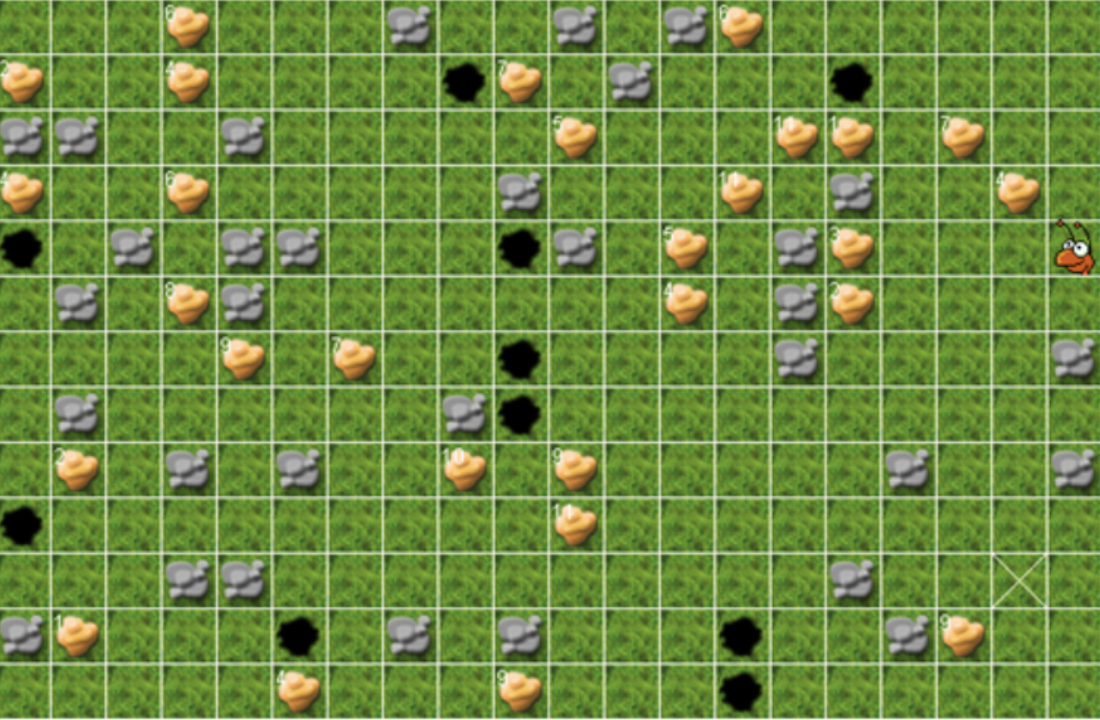
\includegraphics[width=200px]{images/rasterwelt.png}  \end{center}
    \caption{Rasterwelt}
    \label{fig:rasterwelt}
  \end{wrapfigure}
Die ursprüngliche Aufgabenstellung des Wahlpflichtkurses \glqq Agentensysteme\grqq{} ist stark an das Beispiel der \glqq Wumpus-Welt\grqq{} von \cite{wumpus} angelehnt (S.197-200). In einer Rasterwelt, siehe Abb. \ref{fig:rasterwelt}, befindet sich eine Ameise, die auf ihrem Nest spawnt. Ihr Ziel ist es, Futter zu suchen, es aufzusammeln und anschließend zu ihrem Nest zurückzulaufen, um es dort abzulegen. Dabei kann sie sich ausschließlich orthogonal bewegen, Hindernisse können ihren Weg blockieren und sie kann in Löcher fallen, die sie umbringen. Die Wahrnehmung der Ameise beschränkt sich auf die Erkenntnis auf welcher Art von Feld sie sich aktuell befindet sowie dem Futtergeruch oder Gestank orthogonaler Futterquellen respektive Löchern. 

\subsubsection{Problemstellung}
Es gibt zwei entscheidende Gründe, weshalb das ursprüngliche Problemszenario umformuliert werden muss. Zum einen kann das Feedback der Umgebung die Markov-Eigenschaft nicht erfüllen und zum anderen ist die Komplexität des Problems für die tabellarischen Lernmethoden deutlich zu hoch.
\par
Zunächst ist zu verdeutlichen, warum das originale Problem die Markov-Eigenschaft nicht erfüllen kann, die in Kapitel \ref{sec:MP} näher beleuchtet ist. Eine vereinfachte Variante der Informationen, die die Umwelt dem Agenten zukommen lässt, sieht wie folgt aus:
\begin{lstlisting}[language=json,firstnumber=1, label=lst:ursprüngliche Wahrnehmung,caption=bar]
{
    "state": "ALIVE",
    "currentFood": 0,
    "totalFood": 0,
    "cell": {
        "row": 0,
        "col": 10,
        "type": "START",
        "food": 0,
        "smell": 0,
        "stench": 0
    }
}}
\end{lstlisting}
Bei einer solchen Zustandsmodellierung kommt es zu einem ähnlichen Problem wie bei dem, in Kapitel \ref{sec:MP} vorgestellten, Roboter-Beispiel. Angenommen, die Ameise befindet sich auf dem Feld mit den Koordinaten (0,10) und nimmt den Futtergeruch 1 wahr, dann kann die Ameise nicht logisch entscheiden, in welche Richtung sie sich bewegen muss. In einer Konstellation befindet sich das Futter auf dem nördlichen Nachbarfeld, in einer anderen auf dem westlichen Nachbarfeld. Für den Agenten sehen beide Situation identisch aus und er wird sich aufgrund des höchsten Aktions-Nutzens in beiden Fällen für dieselbe Aktion entscheiden.
\par 
Hinzu kommt, dass das Konzept von Fallen genauer gesagt der Fallenerkennung relativ komplex ist und interne Berechnungen benötigt, um logische Schlussfolgerungen ziehen zu können. Bei der ursprünglichen Semesteraufgabe hat der Autor die Umwelt sukzessive in einer internen Repräsentation nachgebaut und anhand von rekursiven Berechnungen Erkenntnisse über mögliche und definitive Fallen zu erhalten.
\par 
Um zusätzliche Algorithmen zu vermeiden, die eine interne Repräsentation pflegen oder Observationen der Umgebung zunächst in valide Markov-Zustände umwandeln, wurde  
auf Fallen als Komponente verzichtet. Zudem ist der Agent nicht mehr in der Lage zu sterben, eine wichtige Änderung hin zu der Konstruktion eines kontinuierlichen Problems.   
\par 
Finalisiert wird die neue kontinuierliche Umwelt dadurch, dass sich nur eine Futterquelle zurzeit auf dem Spielfeld befindet. Legt die Ameise das Futter erfolgreich in ihrem Nest ab, so spawnt eine Futtereinheit erneut in einer zufällig gewählten Zelle.
\par 
Alle Tests wurden auf einer vordefinierten Rasterwelt durchgeführt, bei der die Hindernisse eine spezielle Anordnung haben. Gleichzeitig ist die Spielfeldgröße auf 8x8 Felder reduziert worden. Eine Visualisierung der Rasterwelt  kann der Abbildung \ref{fig:rasterweltNeu} entnommen werden, wobei der Start (das Nest) blau, freie Felder grün und Hindernisse rot markiert sind. Die aktuelle Position der Ameise wird mit einem \glqq A\grqq{} gekennzeichnet, welches die Farbe Schwarz hat, wenn die Ameise kein Futter trägt oder Rot, wenn sie Futter bei sich hat.
\begin{figure}[H]
    \begin{center}
    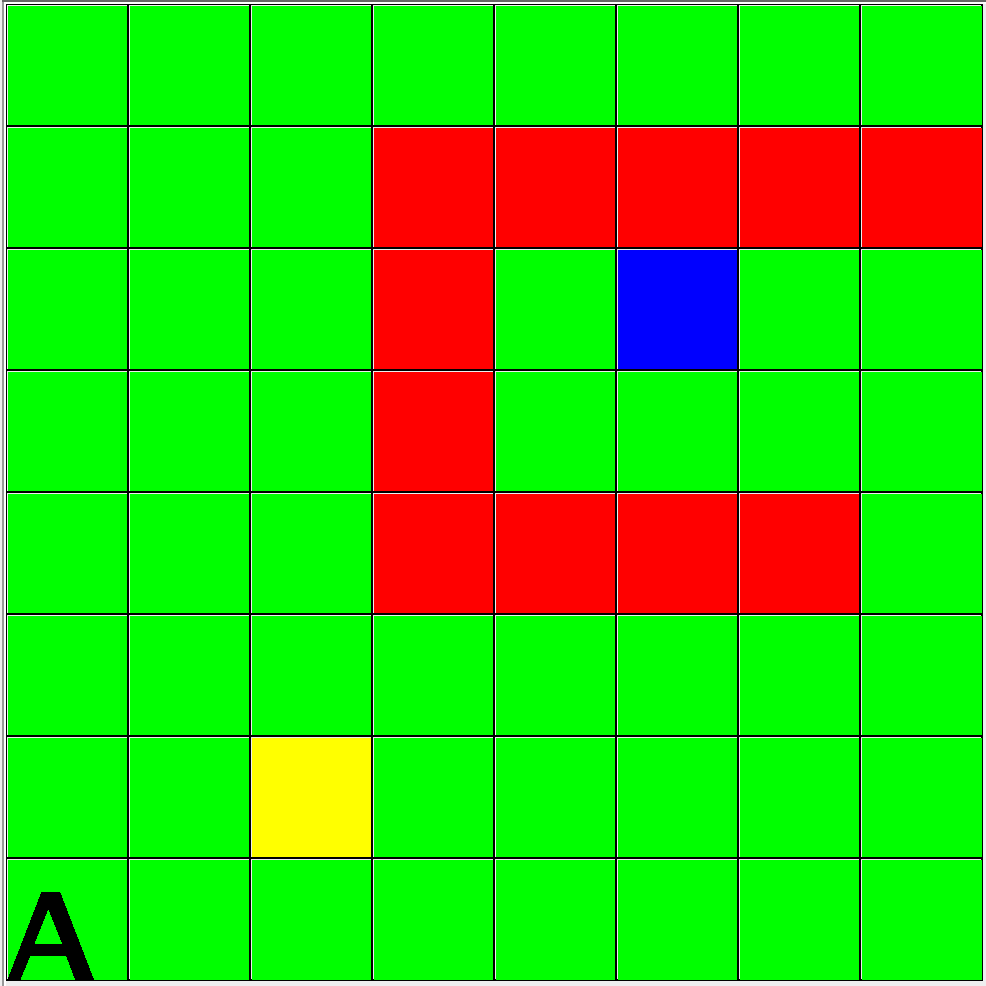
\includegraphics[width=150px]{images/rasterwelt_neu.png}  \end{center}
    \caption{Rasterwelt neu}
    \label{fig:rasterweltNeu}
  \end{figure}

\subsubsection{Zustandsmodellierung}
Die neue Version des \textit{AntGames} wurde im vorangegangen Unterkapitel definiert. Nun beschäftigt sich dieses Unterkapitel mit der Frage, wie eine konkrete Zustandsmodellierung aussehen muss, die die Markov-Eigenschaft bedient und zu optimalen Verhalten führt.
\par 
Das ursprüngliche Konzept von \glqq Gerüchen\grqq{} kann nicht Teil des Zustands sein, da Entscheidung dadurch nicht eindeutig sein können. Nimmt der Agent Futtergeruch wahr, dann befindet sich Futter auf einem der orthogonalen Nachbarfelder. Doch in welche Himmelsrichtung er sich bewegen muss, ist unklar und Bedarf geplantes Erkunden. Bewegt sich die Ameise z.B. nach Norden und bemerkt, dass sie auf keinem Futter steht, dann sollte sie zurückgehen und anschließend das westliche Nachbarfeld überprüfen. Nacheinander potentielle Futterquellen abzusuchen erfordert in jedem Fall das Wissen, welche Felder bereits untersucht worden sind und damit eine Historie besuchter Felder.
\par 
\textit{MDPs} zeichnen sich jedoch gerade dadurch aus, dass Zustandswechsel nicht abhängig von der Historie der gewählten Aktionen ist, wie in Kapitel \ref{sec:MDP} und \ref{sec:MP} beschrieben. Um zu gewährleisten, dass die Historie nicht Teil des Entscheidungsprozesses sein muss, um optimale Entscheidungen zu treffen, wird die gesamte Spielfeldkonstellation als Zustand gewählt. Dieser Ansatz ist inspiriert durch \cite{dqn}, die in ihrer Arbeit vorstellen, wie sämtliche \textit{Atari}-Spiele mithilfe von \textit{Deep Reinforcement Learning} auf menschlichem Niveau gespielt werden können. Als Eingabe oder vielmehr Zustand für den Algorithmus dient die gesamte Pixelkonfiguration des aktuellen Frames. Das Besondere hierbei ist, dass keinerlei Anpassungen an dem Programmcode oder dem Neuronalen Netz vorgenommen werden müssen, um alle 49 \textit{Atari}-Spiele erfolgreich zu meistern.
\par 
Ein Zustand beinhaltet somit die komplette Rasterwelt, d.h. ein zweidimensionales Array, welches alle Zellen mit ihrem jeweiligen Typ speichert (\textit{START, FREE, OBSTACLE}) und der Information, ob Futter auf dieser Zelle liegt. Hinzu kommt die aktuelle Position der Ameise, also \textit{x}- und \textit{}-Koordinate und der booleschen Flag, ob die Ameise Futter trägt oder nicht.
\par 
Intern lässt sich der Zustand folgendermaßen beschreiben:
\begin{equation}
Z_{1} =  \begin{bmatrix} Cell[][]\text{ }world\\
                         antPosition\text{ }(x,y) \\
                        hasFood  \end{bmatrix}
\end{equation}

Der Aktionsraum umfasst die Aktionen \textit{MOVE\_UP, MOVE\_RIGHT,
MOVE\_DOWN,
MOVE\_LEFT,
PICK\_UP und
DROP\_DOWN}. Zusammen mit 2810 möglichen Zuständen für die definierte Rasterwelt ergibt sich die Gesamtanzahl der gespeicherten Aktions-Nutzen von:
\begin{equation}
    G_{AntGame,Z_1} = 16860
\end{equation}

\subsubsection{Belohnungsfunktion}
In diesem Unterabschnitt wird eine abweichende Methode für die Belohnungsfunktion vorgestellt, die den Lernprozess deutlich beschleunigt.
\par
Das Ziel des Agenten ist es, Futter auf direktem Weg zu seinem Nest zu bringen. Gemäß \cite{Sutton1998} und der ähnlichen Modellierung bei dem Jumping Dino Problem, sollte es ausreichen, dem Agenten lediglich eine positive Belohnung von +1 zu übergeben, wenn er das Futter auf sein Nest fallen lässt. Alle anderen Aktionen werden mit +0 belohnt. Und in der Tat, führt diese Modellierung zu einem annähernd optimalen Ergebnis. \glqq Optimal\grqq{} bedeutet im Zusammenhang des \textit{AntGames}, dass die Ameise immer den direkten Weg zum Futter nimmt, es aufhebt und auf unmittelbarem Weg zurück zum Nest läuft, um es abzulegen. Sie stößt nicht gegen Hindernisse oder den Rand der Rasterwelt und legt auf keinem anderen Feld als das Nest ab.
\begin{equation}
    B_{1} =  \begin{bmatrix} 
        FOOD\_DROP\_DOWN\_SUCCESS = +1\\
        DEFAULT\_REWARD = 0           
 \end{bmatrix}
\end{equation}
Diese einfache Modellierung der Belohnung hat jedoch zwei Nachteile. Der erste Punkt ist, dass sie nur annäherungsweise zu dem optimalen Verhalten konvergiert. In Kapitel XX wird eine Methodik vorgestellt, wie gemessen werden kann, ob die Ameise immer den direkten Weg nimmt oder nicht. Vorweggenommen, liegt die durchschnittliche Anzahl an Zeitstempeln pro gesammelten Futter bei optimalen Verhalten bei circa 22,92. \textit{QLearning} erreicht mit der einfachen Modellierung dennoch nur einen Durchschnitt von circa 23,5. Ein marginal erscheinender Unterschied, der jedoch auffällig genug ist, damit ein Mensch ihn ohne Probleme erkennen kann, wenn er der Ameise zusieht. Es fehlt die explizite Modellierung, dass die Ameise nicht \glqq trödeln\grqq{} soll. Dem Labyrinth-Beispiel von \cite{Sutton1998} nachempfunden, erhält die Ameise nach jedem Zeitstempel eine negative Belohnung von -1, was letztendlich dazu führt, dass die Ameise optimal handelt.
\begin{equation}
    B_{2} =  \begin{bmatrix} 
        FOOD\_DROP\_DOWN\_SUCCESS = +1\\
        DEFAULT\_REWARD = -1          
 \end{bmatrix}
\end{equation}
Zwar ist durch diese kleine Änderung sichergestellt, dass die gefundene optimale Strategie $\pi_*$ gleichzeitig auch das optimale Verhalten widerspiegelt, doch bleibt das zweite Problem, die Dauer bis zu der Konvergenz. \textit{QLearning} benötigt rund $600000$ Zeitstempel, um die ersten 1000 Futtereinheiten zu sammeln. Eine detaillierte Belohnungsfunktion ist in der Lage, den benötigten Aufwand drastisch zu verringern. Aktionen, die dem Ziel der Ameise entschieden widersprechen werden zusätzlich negativ belohnt, damit die Ameise schneller lernt, diese in der Zukunft nicht erneut auszuführen. Hierzu zählt beispielsweise das Laufen gegen Wände oder Hindernisse, das Ausführen der Aktion \textit{PICK\_UP} auf einem Feld ohne Futter oder Futter auf einem anderen Feld als das Nest abzulegen. Durch diese Änderungen ist die Ameise während des Lernprozesses in der Lage, die ersten 1000 Futtereinheiten in nur circa $80000$ Zeitstempeln zu sammeln. 
\par
Negative Belohnungen bei Ausführung einer unerwünschten Aktion werden mit dem \textit{DEFAULT\_REWARD} addiert wird, wodurch die -2 zustande kommt. Grund hierfür ist, dass der Agent zwischen der normalen \glqq Bestrafung\grqq{} eines vergangenen Zeitstempels und einer suboptimalen Aktion unterscheiden muss. Die detaillierte Belohnungsfunktion sieht wie folgt aus:
\begin{equation}
    B_{3} =  \begin{bmatrix} 
        FOOD\_PICK\_UP\_SUCCESS = +0\\
        FOOD\_PICK\_UP\_FAIL\_NO\_FOOD = -2 \\
        FOOD\_PICK\_UP\_FAIL\_HAS\_FOOD\_ALREADY = -2\\
        FOOD\_DROP\_DOWN\_FAIL\_NO\_FOOD = -2 \\
        FOOD\_DROP\_DOWN\_FAIL\_NOT\_START = -2 \\
        FOOD\_DROP\_DOWN\_SUCCESS = +1\\
        RAN\_INTO\_WALL = -2\\
        RAN\_INTO\_OBSTACLE = -2 \\
        DEFAULT\_REWARD = -1                  
 \end{bmatrix}
\end{equation}
\\ TODO zusätzlicher Effekt, Diskontierungsfaktor, sonst Rundungsfehler, wenn disc zu niedrig